\documentclass[conference,letterpaper]{IEEEtran}
\IEEEoverridecommandlockouts

\usepackage{amsmath,amssymb,amsfonts}
\usepackage{graphicx}
\usepackage{textcomp}
\usepackage[OT1]{fontenc}
\usepackage{pifont}
\usepackage{multirow}
\usepackage{threeparttable}
\usepackage{booktabs}% 
\usepackage{gensymb}
\usepackage{float}
\newcommand{\tabitem}{~~\llap{\textbullet}~~}

\def\BibTeX{{\rm B\kern-.05em{\sc i\kern-.025em b}\kern-.08em
T\kern-.1667em\lower.7ex\hbox{E}\kern-.125emX}}
\begin{document}
\bstctlcite{IEEEexample:BSTcontrol}

\title{The Cost of Control: Alternative Methods of Preprocessing Demand for HVAC Control}
%
\author{
\IEEEauthorblockN{
Anvitha Ramachandran,
Emily Laus,
Frank Catalano,
Kushagra Srivastava
}
\IEEEauthorblockA{
\textit{Integrated Concentration in Science Program at UMass Amherst}\\
Amherst, MA \\}
}

\maketitle

\begin{abstract}
Heating, Ventilation, and Air Conditioning (HVAC) systems are essential for indoor comfort, but the systems account for more than $40\%$ of energy consumption in a typical industrial building. 

Our research simulates a commonly used HVAC controller and demonstrates the effects of two methods of preprocessing a curve of temperature setpoints for controller input on the energy consumption and cost of heating the room according to the controller's instructions.
\end{abstract}

\begin{IEEEkeywords}
thermostats, energy consumption, HVAC, simulation
\end{IEEEkeywords}

\section{Introduction}
\label{sec:Introduction}
As of 2022, approximately $3.9\%$ of global greenhouse gas emissions and 10\% of global electricity usage overall have originated from air conditioning systems \cite{woods_humiditys_2022}. Furthermore, according to a report by the International Energy Agency (IEA), targeting specific inefficiencies of air conditioning systems is paramount to reducing the total energy consumption of office buildings, since air conditioning contributes to 20\% of their electricity use around the world \cite{IEA_Future}. A specific but costly example of an inefficiency in air conditioning systems (and even HVAC systems as a whole) involves the patterns and peaks of an HVAC demand curve, which is formed by the controller that designates the desired temperatures of a building and which dictates the conditions that are used to heat or cool a room (such as the temperature of the air entering the room from the radiator). Depending on how the shape of this curve compares to the specifications of the room and the abilities of the HVAC system, it is possible that the demand curve will demand more from the HVAC system than is necessary to maintain a desired temperature in the room. Fortunately, previous studies have shown that it is possible to optimize the demand curve (thus the energy output of the HVAC system) with filters on the controller, changing the demand curve's shape \cite{6687952} . Our research explores this potential through computer simulation, modeling the controller of an HVAC system and the temperature of the room it controls. With this simulation, we analyze the relationship between an HVAC controller, its applied filters, and the energy consumption of the HVAC system. 

\section{Background}
\label{sec:Background}
\subsection{Key Terminology}
\begin{enumerate}
    \item \textbf{HVAC:} Heating Ventilation and Air Conditioning, which is a system used to regulate the temperature of a room or building.
\item \textbf{Demand Curve}: The signal representing what temperature the building manager is setting the room to as a function of time
\item \textbf{Controller:} The device that controls the temperature of air that is going into the room
\item \textbf{Preprocessing:} The work that is done on inputs to a system before feeding them into the system.
\item \textbf{Filter:} A system that takes a raw signal as input and modifies it to aid in the usage of the signal elsewhere in the system.

\end{enumerate}

\subsection{Measures for Designing HVAC Systems}
In order to develop a representative simulation for determining the impact of inaccurate thermostats on the controls for maintaining the temperature of a room, we had to analyze what fundamental features for an HVAC system would go into a simulation of the controls. For example, in a report by Philip Luu for Texas Instruments \cite{Luu2021} regarding the use of one of their sensors for an HVAC system, they describe the general structure of an HVAC system. This is essentially a thermostat with sensors and user control as well as a central controller for controlling the behavior of the air in the room. After detecting a change in the controller signal value [which occur because of changes in the temperature of the mixed-air chamber or changes in the desired temperature], air must be brought into the mixed air chamber to be treated to flow through the supply duct. For enthalpy economization, sensors are placed in the outdoor and return air ducts to determine the air with lower enthalpy to be brought in to the mixed air duct and then heating/cooling coils treat it to be the appropriate temperature and be blown through the room. 

The study from Asim et al. about the sustainability of HVAC units \cite{ijerph19021016} corroborates this, describing a similar valve structure with heating and cooling coils to modify the temperature of the air. It suggested a variety of modification methods, each affecting separate parts of the system, which implies a modular construction to target sore points. It describes targeting a sore point via retrofiting as upgrading "mechanical systems" such as the thermostats and control algorithms in older buildings for retro fitting, and "establishments of the relationship between the investment of retrofitting and the sustainability performance", and a modular configuration would be conducive to drawing such comparisons for retrofitting prior to evaluating their benefits.

Lin et al. of University of Florida have published two papers, one of which is regarding the impact of lowering the frequency of the demand response curve due to the flexibility that the demand of an HVAC system would allow, providing ancillary services [i.e. managing the balancing act between consumers and generators] for a building \cite{6687952}. In these papers \cite{6687952, 7171796}, Lin et al. determined the reduction in energy consumption by consulting with field data from Pugh Hall at the University of Florida in order to compare their results to that data for determining the energy consumption and cost savings. They found that demand for ancillary services can be met by using a band pass filter, resulting in 43GW of reserve energy when using passband frequencies corresponding to 3-60 minutes as opposed to 3-30 minutes. 


\subsection{Energy Efficiency versus Optimal Comfort}

Our goal for this research is to maximize energy efficiency in commercial HVAC Systems while maintaining the comfort of occupants. For the purposes of this study, the term "occupant comfort" is defined as maintaining the room temperature at an optimal level with respect to what values were set on thermostats for the HVAC system.

We plan to model the HVAC system's controllers, and tweak its functioning a bit in a way which would yield higher energy savings, while maintaining occupant comfort. The controller is the main sensor which takes in input from all other sensors, and directs all other HVAC Components to function efficiently. In an interview with Peter Volpe, Electrical Engineer at the University of Massachusetts Amherst Central Heating Plant, he mentioned that the majority of the university uses the Johnson Controls FX20/FX60 controllers for their HVAC Systems. These controllers rely on the PRAC+ System\cite{johnsoncontrolsOpenBlueBuilding}, which is an adaptive control algorithm that automatically tunes a standard Proportional Integral Derivative (PID) controller.

PRAC+ sets tuning parameters to a range, otherwise known as thermal setpoints, and aims to keep the room temperature under this range. These values are set by the building manager, and are intended to keep the building consistently at the given temperature. For example, a temperature setting of 70\textdegree F on the whole system may co-relate to a thermal setpoint of 68\textdegree F on the low end, and 72\textdegree F on the high end. This would mean that the HVAC system would keep the temperature in between this range. 

It is crucial for the HVAC System to maintain an optimal temperature to achieve occupant comfort, and get to the most efficient energy consumption to lower the costs. Our model would achieve energy efficiency, while ensuring to maintain room temperature between these setpoints.

\section{Objective}
\label{sec:Objective}
Our goal is to create a comparative tool to analyze the costs associated with demand preprocessing of HVAC controllers. We plan on using EWMA-based filtering of the setpoint curve and frequency-based filtering to account for the response time and reduce energy wastes regarding unrealistic setpoint expectations. 

\section{Research Question}
\label{sec:Research Question}

What are the energy and cost savings associated with alternative methods of preprocessing demand handling in the controller for heating, ventilation and air conditioning (HVAC) systems?


\section{Hypothesis}
\label{Hypothesis}
We hypothesize that using a lower frequency of demand curve signal [i.e. one with a dead time of 2 times that of the typical] and a midway value for EWMA filtration (0.9 weighting of the previous value)] will lead to the scenario that optimizes for occupancy comfort while also consuming less energy than the standard values [EWMA=1, demand curve has been filtered to have the period be equivalent to that of our dead time]. We calculate the typical scenario's dead time in Section \ref{sec: Dead Time Calculation}, and it is roughly 13 minutes and 20 seconds, which corresponds to an update frequency of 4.5 updates per hour.

\section{Methods}
\label{sec:Methods}

\subsection{Simulation Block Diagram}
\begin{figure}
    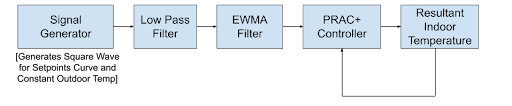
\includegraphics[scale=0.47]{blockdiagram.png}
    \caption{Block diagram representing the key mechanics of our simulation.}
\end{figure}


The block diagram demonstrates the processing pipeline to go from a demand curve to the resultant temperature as a result of the PRAC+ controller. This processing pipeline is recreated in Simulink to demonstrate the measures that would be taken to translate the preprocessed setpoints signal into the actual temperature of the room over the course of the two hours that the simulation is for. 

The pipeline starts with a signal generator, which is intended to emulate the constant outdoor temperature as well as the setpoint curve. The low pass filter is fed a specific cutoff frequency that we determine in the testing parameters, based on the typical dead time of around 13.5 minutes for the controller. We analyze the effects of filtering the curve by attenuating all frequencies above 2.25 updates per hour, 4.5 updates per hour, and 9 updates per hour, and the demand curve fed in all three cases is identical and at a frequency of 18 updates per hour so that we can compare the filters' efficacy with equal demand curves. The EWMA Filter is a smoothing filter that is based on the weighting of previous values’ effect on the data. We apply the filter, $f_t=\alpha P_t + (1-\alpha)f_{t-1}$, where $f_t$ is the value at any point following the first one and $\alpha$ is the forgetfulness factor, or how much the current data point is weighted with respect to the previous one. This is the parameter b in the setpoint weighting for the PRAC+ controller, as per the setpoint weighting module in their specification \cite{johnsoncontrolsSetpointWeighting}. The next block is the PRAC+ controller itself, which is recreated according to the specification available in their PID controller outline \cite{johnsoncontrolsPID}. Lastly, after determining the temperature of air that is sent through the valves to moderate the temperature in the room, the resultant temperature of the room is calculated using the equations in Section \ref{sec:Equations}.
\begin{figure}
    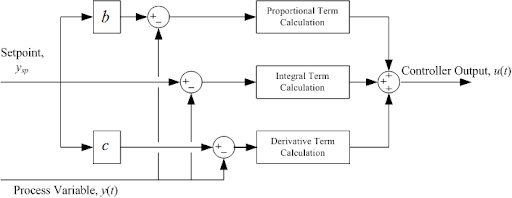
\includegraphics[scale=0.48]{prac.png}
    \caption{Setpoint weighting in the PRAC+ controller.}
\end{figure}

\begin{figure}
    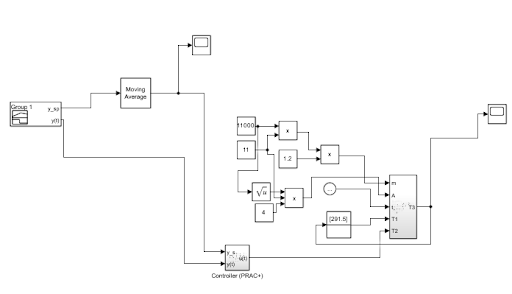
\includegraphics[scale=0.48]{simulink.png}
    \caption{The block diagram as it translates to the Simulink subsystems.}
\end{figure}



\subsection{Dead Time Calculation}
\label{sec: Dead Time Calculation}
In order to calculate the dead time in a typical scenario for the Johnson Controls PRAC+ Controller, we run a simulation that takes one step input from 65\degree F to 72\degree F as opposed to the square waves that we run the experiments in the simulation with, and an outside temperature of 65\degree F that is constant. This lets us determine the amount of time between when the "jump" occurs and when the resultant temperature hits the threshold specified by the PRAC+ controller [within 0.04 times the delta between the setpoint and the outdoor temperature], so roughly 0.28\degree F within the 72\degree F setpoint. We define $L$ as an input to be the length of the duct leading up to the room in meters, and we use the Air Conditioning Contractors of America [ACCA] and the National Renewable Energy Laboratory [NREL] guidelines of 700 feet per minute, or around 3.5 m/s \cite{Burdick2011} as a typical duct speed to calculate the total time it takes for the air to be heated up and then sent to the room via the duct, which is defined by the PRAC+ Controller specification as dead time, and refers to the amount of time the system takes to respond to the controller's specification.

\begin{figure}
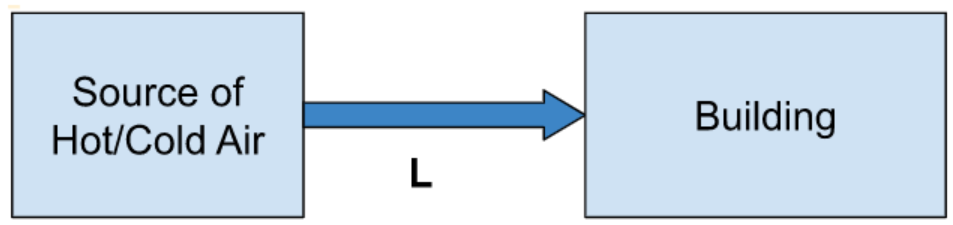
\includegraphics[scale=0.5]{length.png}
    \caption{Figure describing how we determined the latter part of the dead time in the calculation}
\end{figure}


\subsection{Data Collection}
\label{sec: Data Collection}
The inputs with respect to room size and duct length and input setpoint signal are held constant, whereas the filter values are stepped from 2.25 updates per hour to 4.5 updates per hour to 9 updates per hour for the cutoff frequency. The EWMA $\alpha$ values are stepped from 0.75 to 0.95, with 0.97 and 0.99 to showcase the rapid change in the waveform for $\alpha$ between 0.9 and 0.1 compared to the other gradually stepped values. 

\subsection{Variables}
The following variables are used in our equations and with the 
\begin{enumerate}
    \item $P = \frac{Q}{t}$ power required
\item $Q$ energy required
\item $t$ time passed
\item $k$ insulation value of wall
\item $x$ thickness of wall
\item $A_W$ surface area of wall(s) combined
\item $A_R$ surface area of radiator(s) combined
\item $T_h$ hotter temperature
\item $T_c$ colder temperature
\item $T_1$ temperature before specified time $t$
\item $T_2$ temperature after specified time $t$
\item $T_o$ outdoor temperature
\item $\epsilon = 1$ emissivity
\item $\sigma$ Stefan-Boltzmann constant
\item $m_a$ mass of air
\item $c_V$ specific heat (with constant volume)
\item $\alpha$ EWMA filter value in our equation for it
\item $b$ EWMA filter variable name in the PRAC+ inputs
\end{enumerate}

\subsection{Equations and Calculations}
\label{sec:Equations}
To model the temperature of our modeled room over time along with the energy consumed to adjust or maintain its temperature, we incorporated three thermodynamic equations into our model, the Law of Radiation, the Law of Conduction, and the relationship between heat transfer (energy) and temperature change of a substance: 

\begin{enumerate}
    \item \textbf{Law of Radiation}: $P_R=\epsilon\sigma(T_h^4-T_c^4)A_r$
    \item \textbf{Law of Conduction}: $P_C=\frac{-kA_w(T_h-T_c)}{x}$
    \item \textbf{Relationship between Heat Transfer and Temperature Change}: $Q=m_ac_V(T_h-T_c)$
\end{enumerate}

The Law of Radiation determines the rate at which heat enters our modeled room through the HVAC radiator(s), the Law of Conduction determines the rate at which heat escapes the room through its walls, and the relationship between heat transfer and temperature change determines the total energy required to change the temperature of our room. As these equations demonstrate, the temperature of our room constantly changes over time, meaning that any power output or energy consumption is dependent on time. As such, for our model to account for this time-dependence, the simulation repeatedly runs this calculation, which combines all three of our previous thermodynamic equations:

\textbf{Time-Dependent Temperature Change}:

$T_2=\frac{m_ac_VT_1 + \epsilon\sigma(T_h^4-T_1^4)A_rt - kA_w(T_1-T_o)\frac{t}{x}}{m_ac_V}$

We required our simulation to make this temperature calculation every second ($t=1$), meaning that the model simulated the temperature of the room within 1-second precision. This relationship allows us to produce temperature versus time graphs, shown in Section \ref{sec:Results}.

\subsection{Assumptions}
\label{sec: Assumptions}
As per the Johnson Controls specification guide for the controller \cite{johnsoncontrolsPRAC}, the simulation we build represents a system operating under the following assumptions:
\begin{enumerate}
    \item The system is non-redundant, i.e. there are not multiple controllers in the room that are operating at fractions of their capabilities as this impacts the accuracy of the automatic tuning that is done on the system.
    \item All demand to heat/cool the air to get the room to a certain temperature is met.
    \item Air systems must be able to provide the appropriate capacity of hot/cold air to the room.
\end{enumerate}

At the same time, other assumptions were made for our simulation in order to simplify and specify our thermodynamic calculations:
\begin{enumerate}
\item No air or heat is lost through the ducts between our energy source and modeled room (shown in Figure 2).
\item The air traveling through the ducts has a constant velocity, such that we can model its travel time from source to room as if it is a solid substance traveling with a constant velocity from one point to another (considering the effects of gravity to be negligible).
\item Our model can provide an accurate representation of temperature change without incorporating windows or doors into the room's structure.
\item Because the simulation only runs a model for a couple of hours at a time, we assume the temperature outside of the room ($T_o$) to be constant. Furthermore, for this simulation, we assume the outdoor temperature to be 65\degree F at all times (though in future research, this outdoor temperature could be changed to observe the impact of outdoor temperature on our current results).
\end{enumerate}

\subsection{Outputs}
\label{sec: outputs}
For our output of the simulation, we get a curve which we call $T_2$ that is temperature (K) versus time (s) that represents the actual temperature in the room due to the PRAC+ controller determining the temperature of the air that flows through the ducts and then the dissipation of the air in the room over time. We calculate the power consumption using the assumptions from Section \ref{sec: Assumptions} by determining the input power from the equation in \ref{sec:Equations} to get power needed to heat/cool the temperature of the air in the duct to that stated by the controller, as that is the predominant effect on the power consumption of the system that is affected by the setpoint curve preprocessing that we are analyzing in the study.

\section{Results and Analysis}
\label{sec:Results}
\subsection{Results}
    To visually represent the effects of EWMA filters and update frequency in our HVAC controller, we produced two types of graphs from our simulation:

\begin{enumerate}
\item Temperature Over Time
\item Power Output Over Time
\end{enumerate}

    First, the Temperature Over Time graphs depict the demand curve designated by the controller (orange) and the actual temperature of the room (blue), based on the specifications of EWMA filters and update frequency.
    Second, the Power Output Over Time graphs depict the power that is radiated from our radiators in the modeled room, dependent on the current temperature of the room and the temperature of the air emitted from the radiators. It is important to note that this is \textit{not} the amount of power actually being used to heat up the room, rather it is the rate of heat transfer from the emitted air of the radiator to the air in the modeled room. As such, this type of figure does not provide quantitative information for power consumption from our HVAC system, rather it visually demonstrates the distance between the temperature of the air from the radiator and the temperature of the room (based on the Law of Radiation, shown in \ref{sec:Equations}).
\begin{figure}[H]
    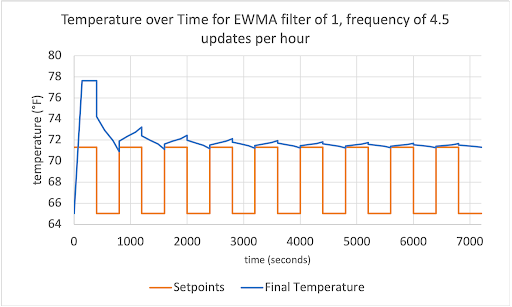
\includegraphics[scale=0.48]{tempcontrol.png}
    \caption{The resultant temperature over time for the control scenario, where EWMA = 1 and the frequency = 4.5 updates/hour. These values represent the average HVAC controller's specifications.}
\end{figure}
\begin{figure}[H]
    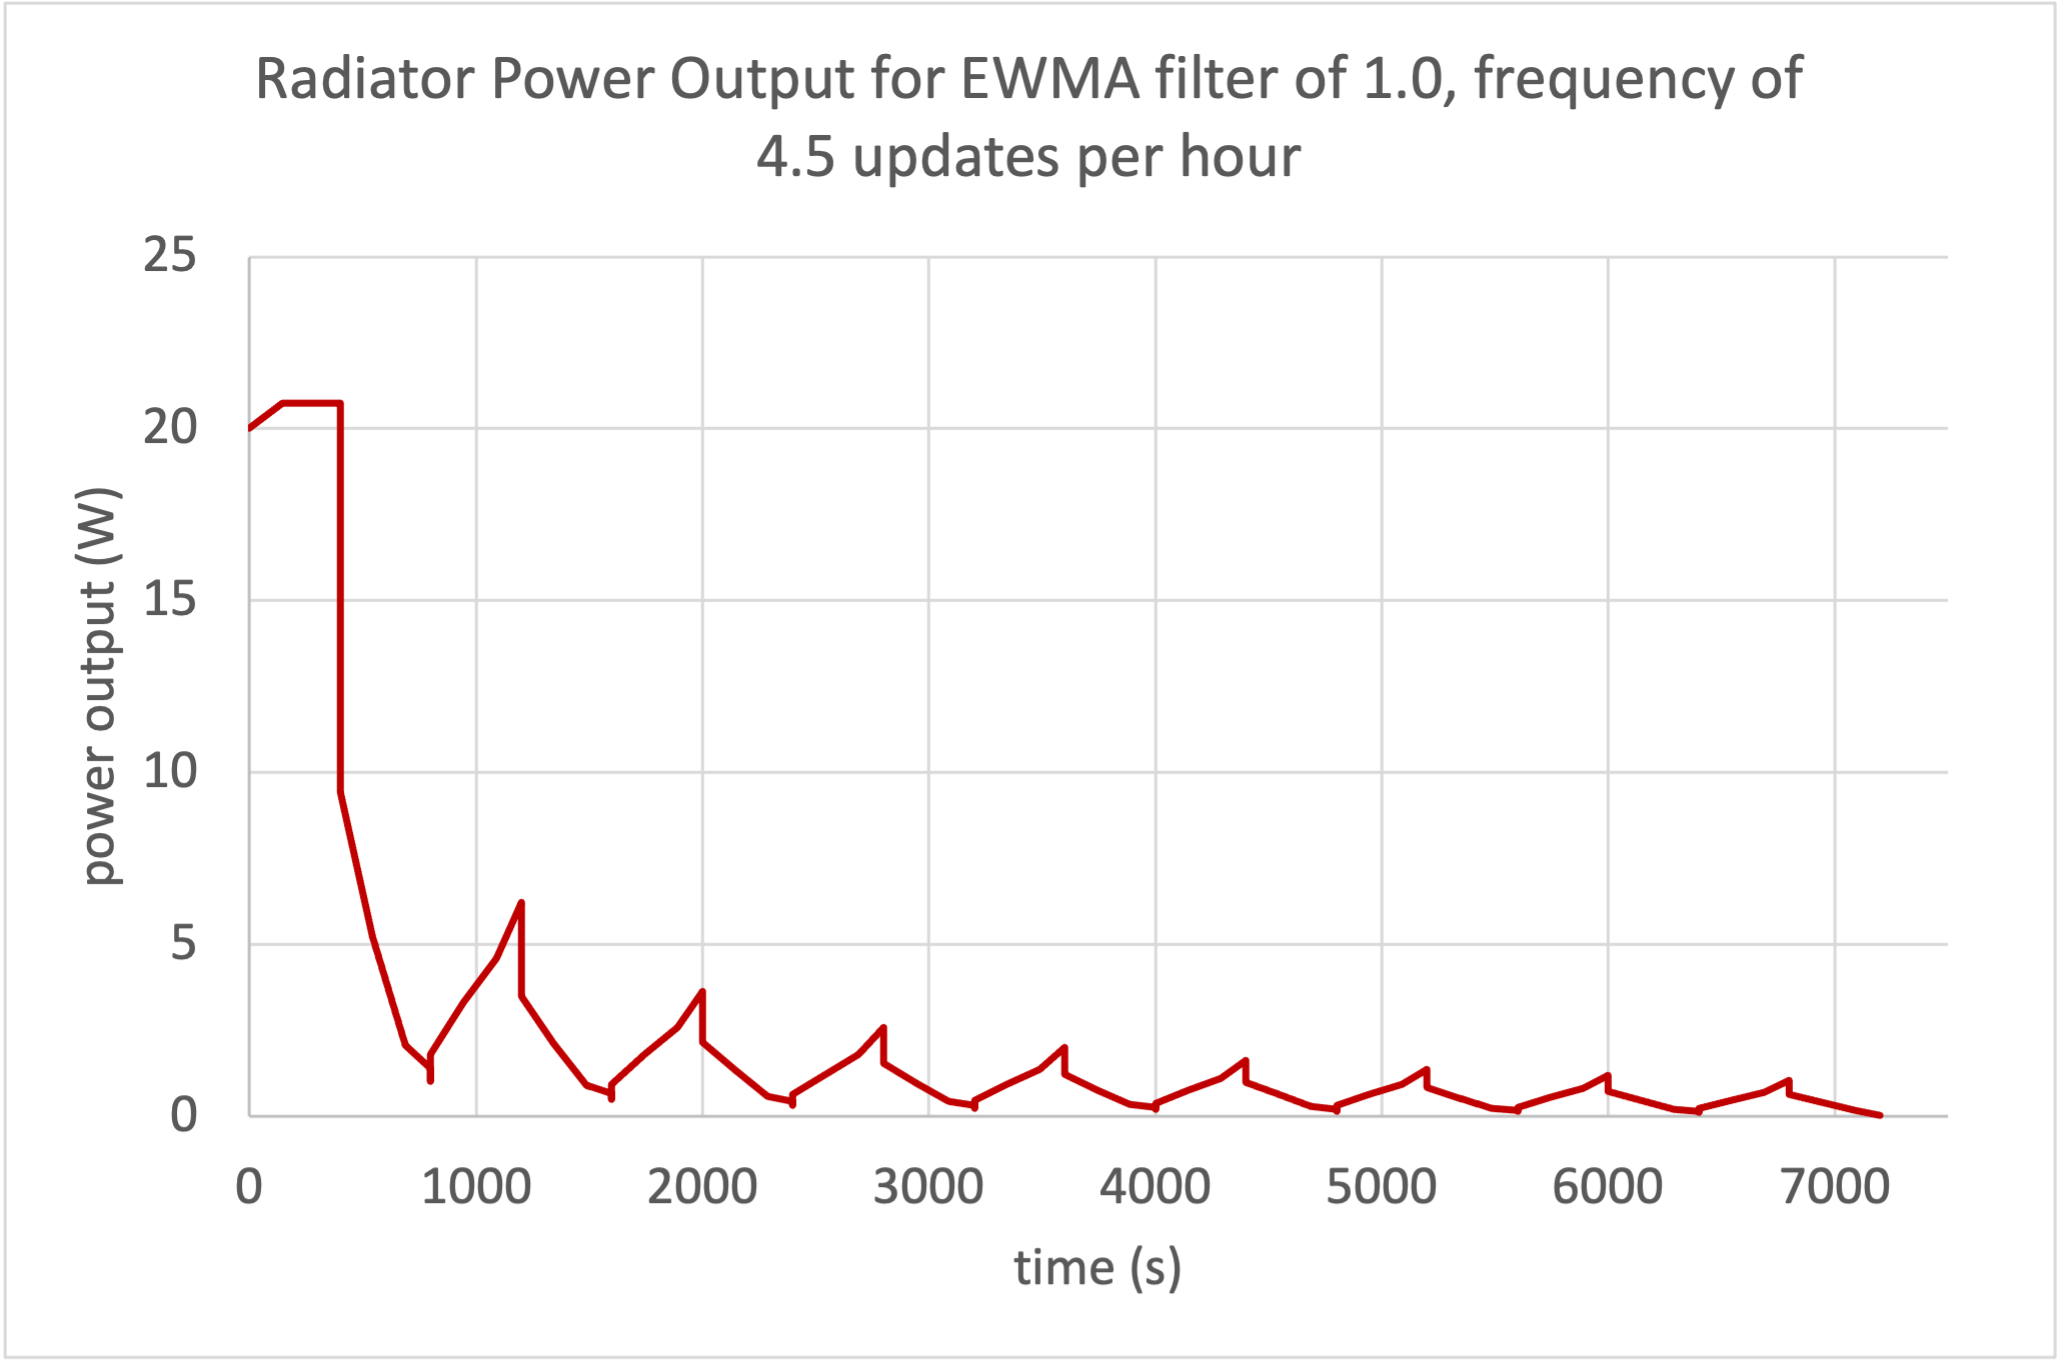
\includegraphics[scale=0.48]{powercontrol.png}
    \caption{The resultant power over time for the control scenario, where EWMA = 1 and the frequency = 4.5 updates/hour. These values represent the average HVAC controller's power consumption.}
\end{figure}
\begin{figure}[H]
    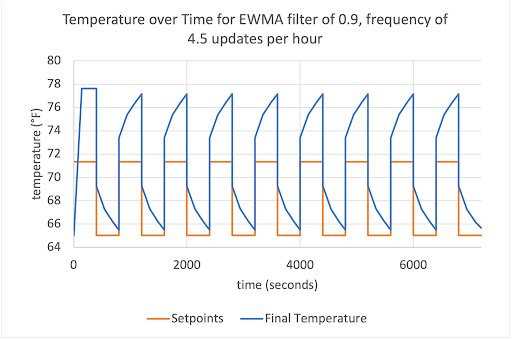
\includegraphics[scale=0.48]{tempworst.png}
    \caption{The resultant temperature over time for the worst scenario, where EWMA = 0.9 and the frequency = 4.5 updates/hour. This results in the highest gradients of room temperature.}
\end{figure}
\begin{figure}[H]
    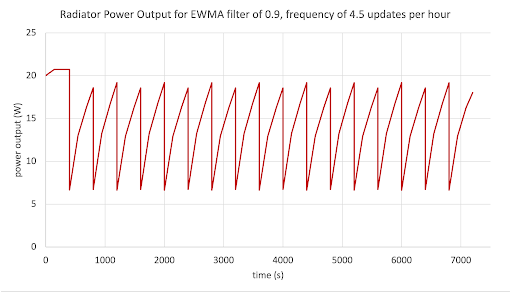
\includegraphics[scale=0.48]{powerworst.png}
    \caption{The power over time for the worst scenario, where the EWMA = 0.9 and the frequency = 4.5 updates/hour. There is significantly higher power usage in this scenario.}
\end{figure}
\begin{figure}[H]
    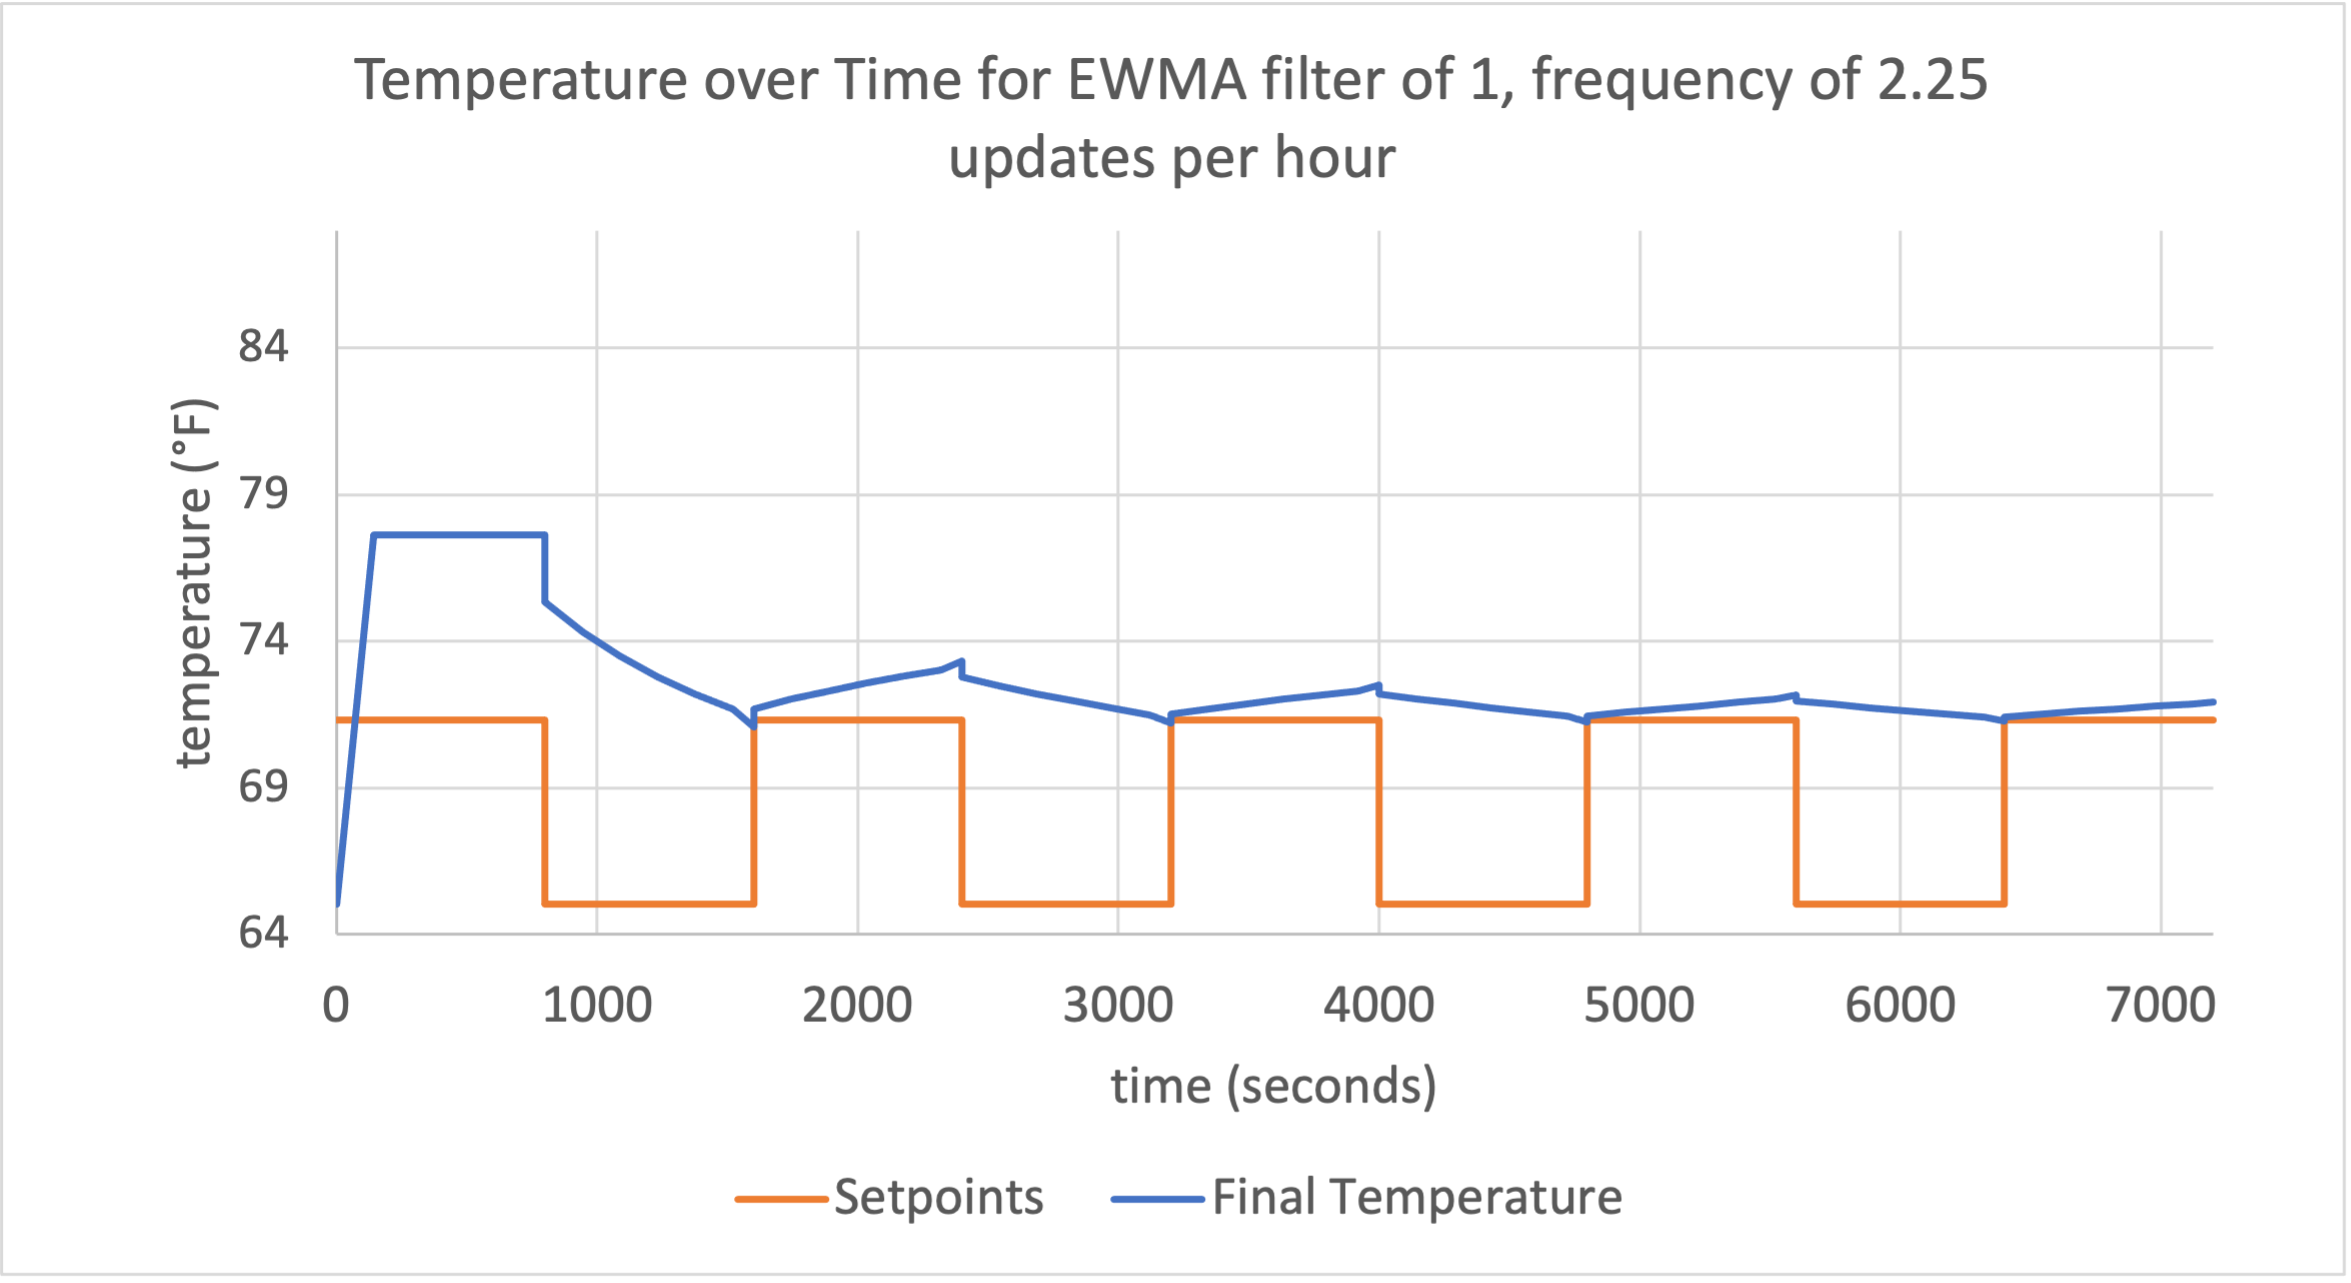
\includegraphics[scale=0.48]{tempbest.png}
    \caption{The resultant temperature over time for the best scenario, with EWMA = 1, and frequency = 2.25 updates/hour. The temperatures stay very much within the setpoints, delivering occupant comfort.}
\end{figure}
\begin{figure}[H]
    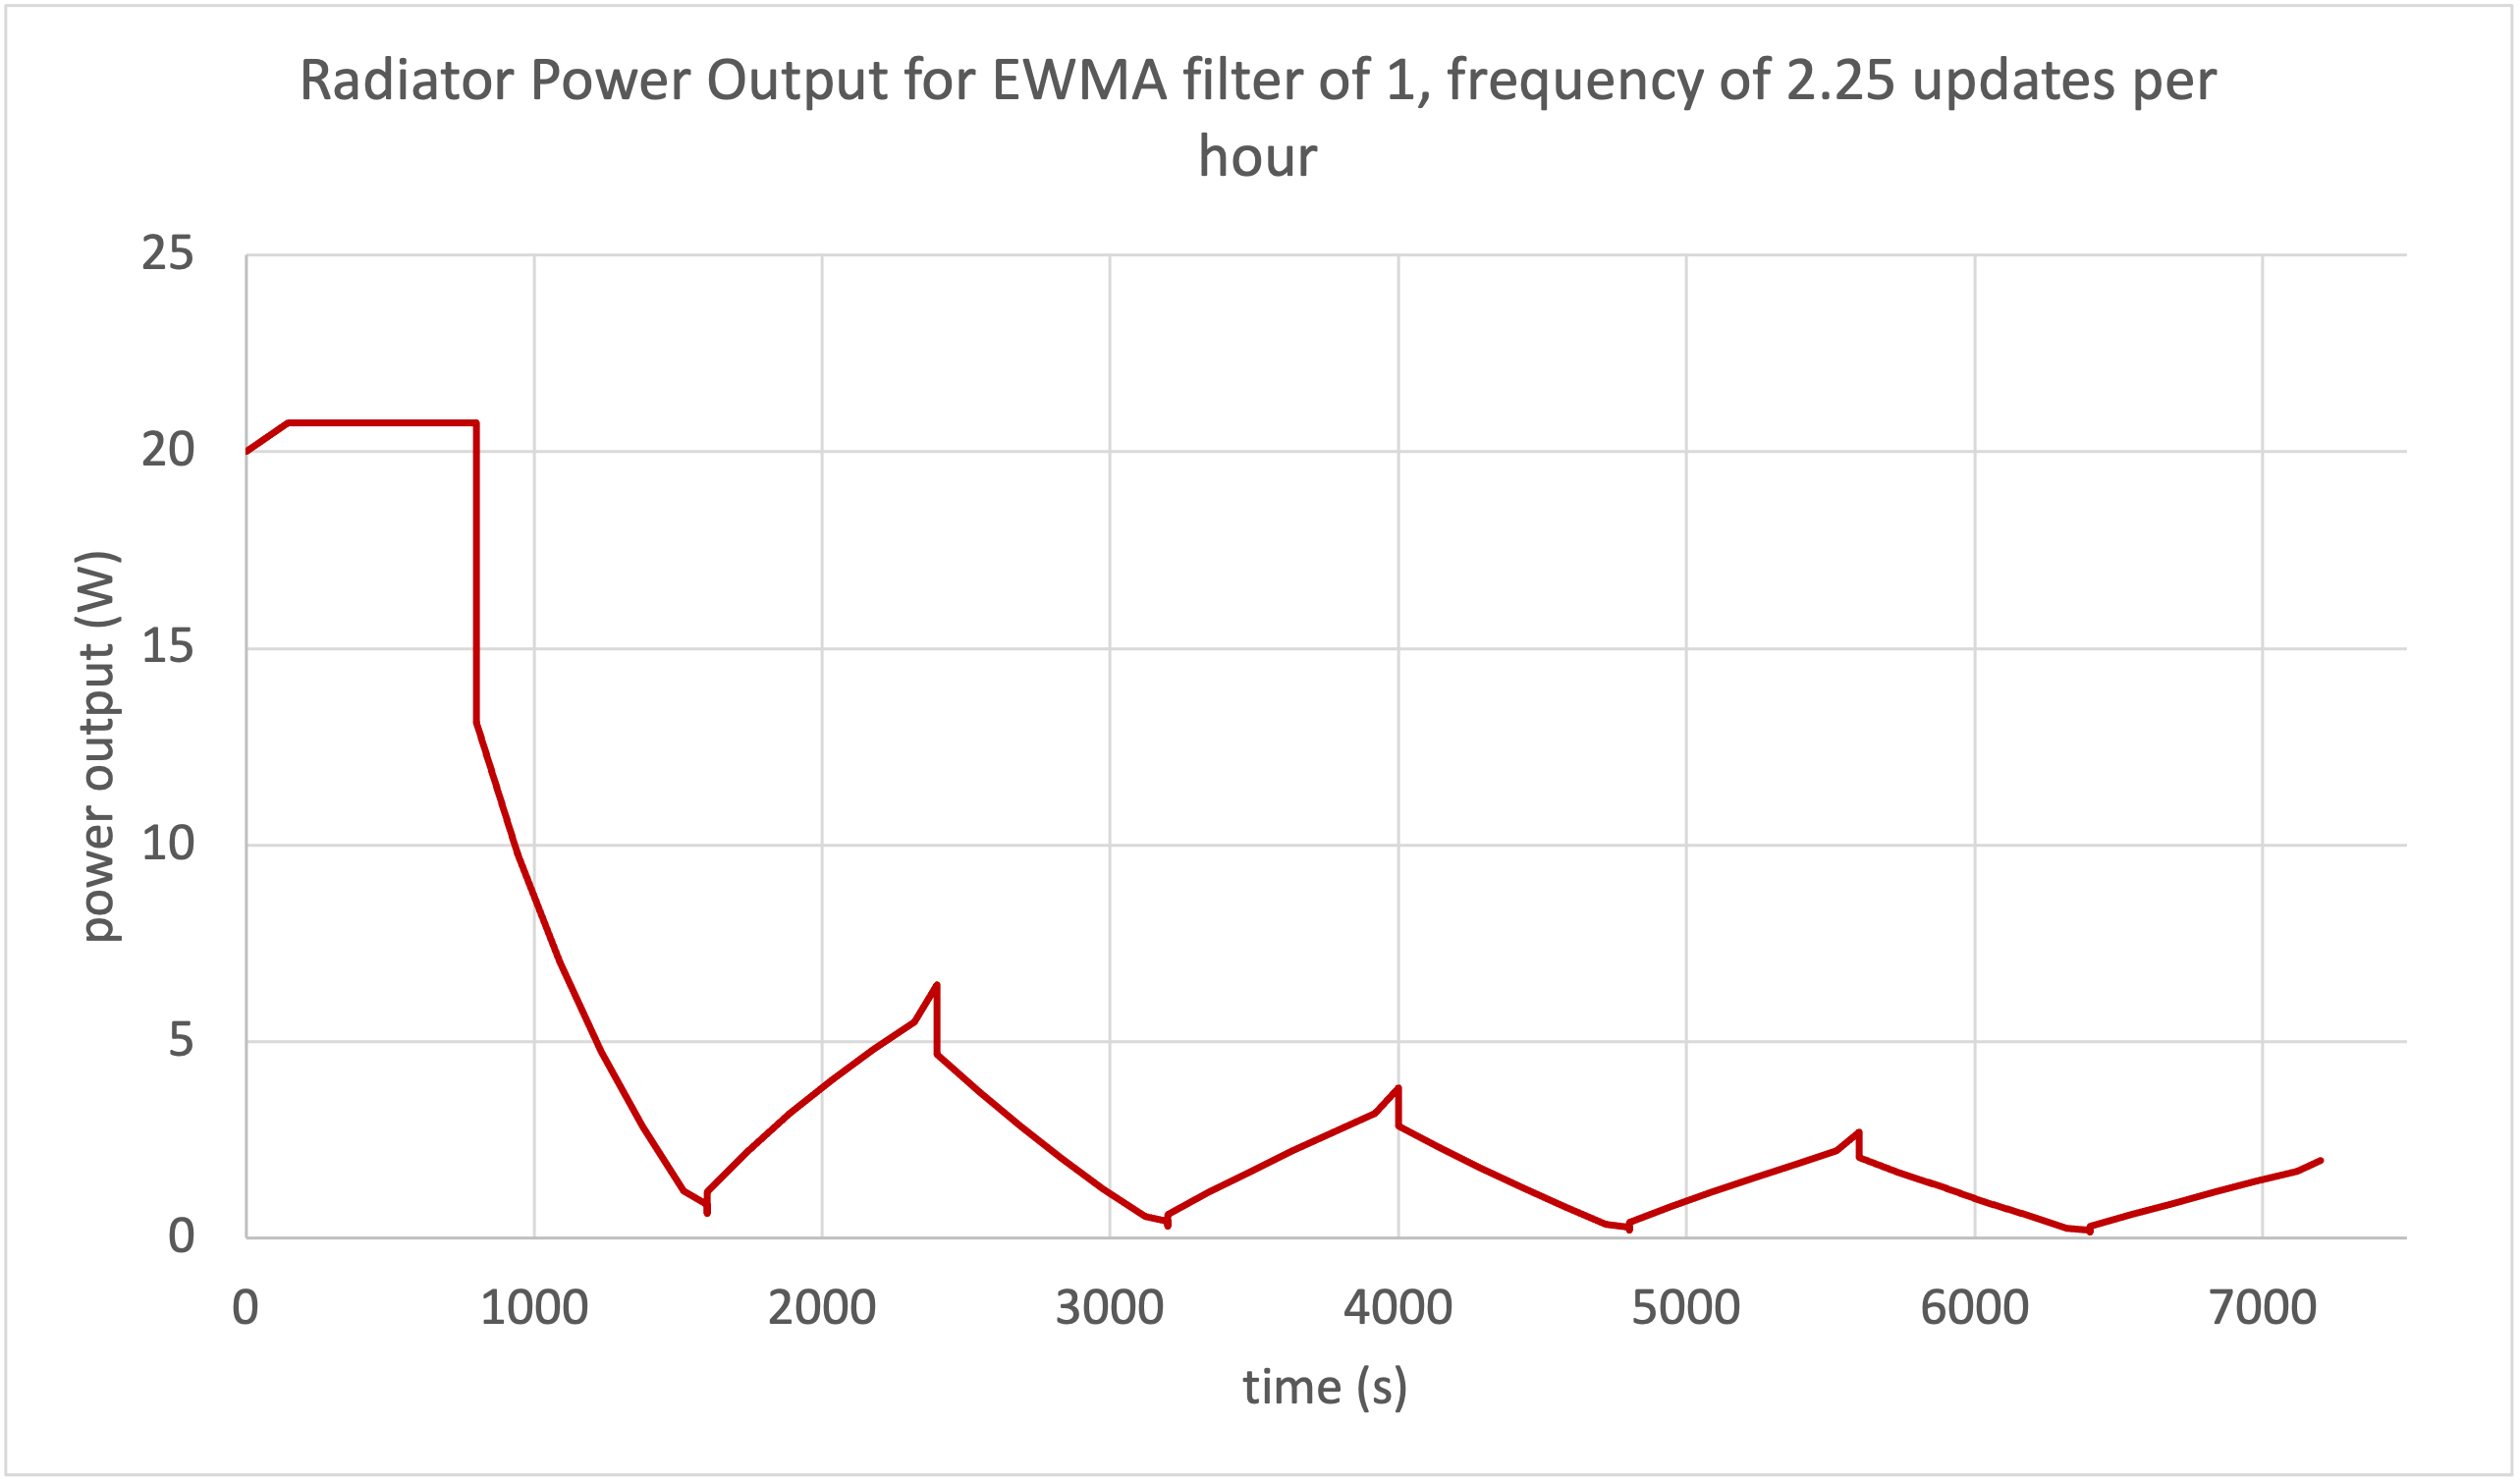
\includegraphics[scale=0.48]{powerbest.png}
    \caption{The power over time for the best scenario, with EWMA = 1, and frequency = 2.25 updates/hour. }
\end{figure}

\subsection{Analysis: Energy and Cost}
\label{sec:Analysis}
Using the temperature versus time trends displayed in our \ref{sec:Results} section and the relationship between heat transfer and temperature change (shown in the \ref{sec:Equations} section), we can calculate the approximate energy consumed over the course of two hours to heat our room with the specified controller variables (EWMA filter and update frequency). At the same time, we use a cost-analysis of UMass Amherst's utilities to approximate that the average blended cost of energy on their campus per kilowatt-hour (kWh) is \$0.0675. These approximations lead us to our calculated energy and financial costs for the three cases of EWMA filter and update frequency graphed in \ref{sec:Results}. These calculated results are shown in the table below:
\begin{figure}[H]
    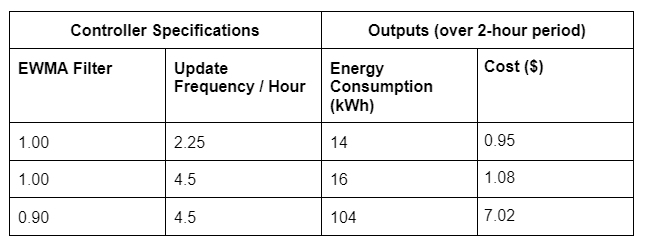
\includegraphics[scale=0.64]{analysis.png}
    \caption{The financial analysis of our three scenarios from Section \ref{sec:Results}}
\end{figure}

These results demonstrate that if EWMA = 1, we save a small amount of energy and money by cutting the update frequency in half. However, if we choose to maintain the update frequency but reduce our EWMA filter to 0.9, our energy and cost is multipled by \textit{more than 7 times}. These results on their own are suggestive of the effects of EWMA filter and update frequency, but to solidify our findings, we account for the energy and cost consumption of 24 different cases, shown in the following sections. In these cases, the EWMA filter can be either 1.00, 0.99, 0.975, 0.95, 0.90, 0.85, 0.80, or 0.75. Furthermore, the update frequency for any of these filters is either 2.25, 4.5, or 9 updates per hour.

\subsection{Impact of EWMA Filtering}
In this extended investigation, we first explore the impact of the EWMA filter by modeling the energy consumption versus filter, creating a clustered bar chart with each frequency represented by its own color (pink for 2.25, green for 4.5, and purple for 9). This leads to our clustered bar chart and trendline chart displayed below:
\begin{figure}[H]
    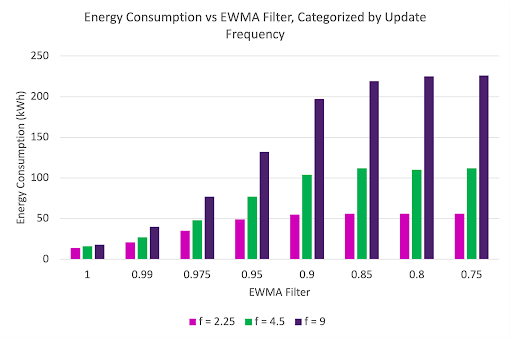
\includegraphics[scale=0.48]{barewma.png}
    \caption{The energy consumption of the HVAC system versus the specified EWMA filter, color-categorized by the three possible frequencies.}
 \end{figure}   
 \begin{figure}[H]
    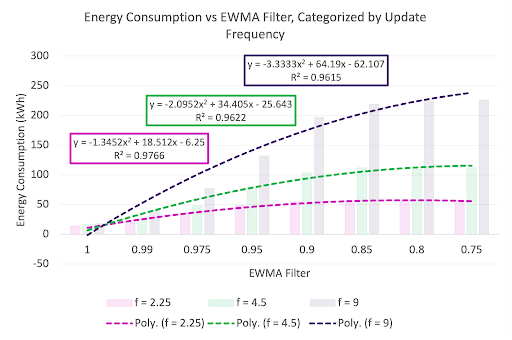
\includegraphics[scale=0.48]{lineewma.png}
    \caption{The trendlines of the energy versus EWMA filter graph, consisting of second-order polynomials to represent the approximate trend of energy consumption with lowering EWMA filter, separated by frequency.}
\end{figure}
These two figures can lead to at least two conclusions:
\begin{enumerate}
\item For any specified frequency, energy consumption increases as EWMA filter decreases from 1.00 to 0.75. This energy increase somewhat resembles a logarithmic function, appearing to possibly "peak" at a certain energy consumption. However, further studies with a wider range of EWMA filters would be necessary to be certain with this observation.
\item A higher frequency leads to a greater dependence on EWMA filter, meaning that the change in energy consumption is dependent on the combination of EWMA filter and update frequency.
\end{enumerate}

\subsection{Impact of Update Frequency}
To continue our extended investigation, we next explore the impact of update frequency by "reversing" the roles from our previous figures, clustering our bars by update frequency and coloring them by EWMA filter (in a rainbow pattern, with red representing EWMA = 1 and brown representing EWMA = 0.75). Through this process, we obtain the two figures shown below:
\begin{figure}[H]
    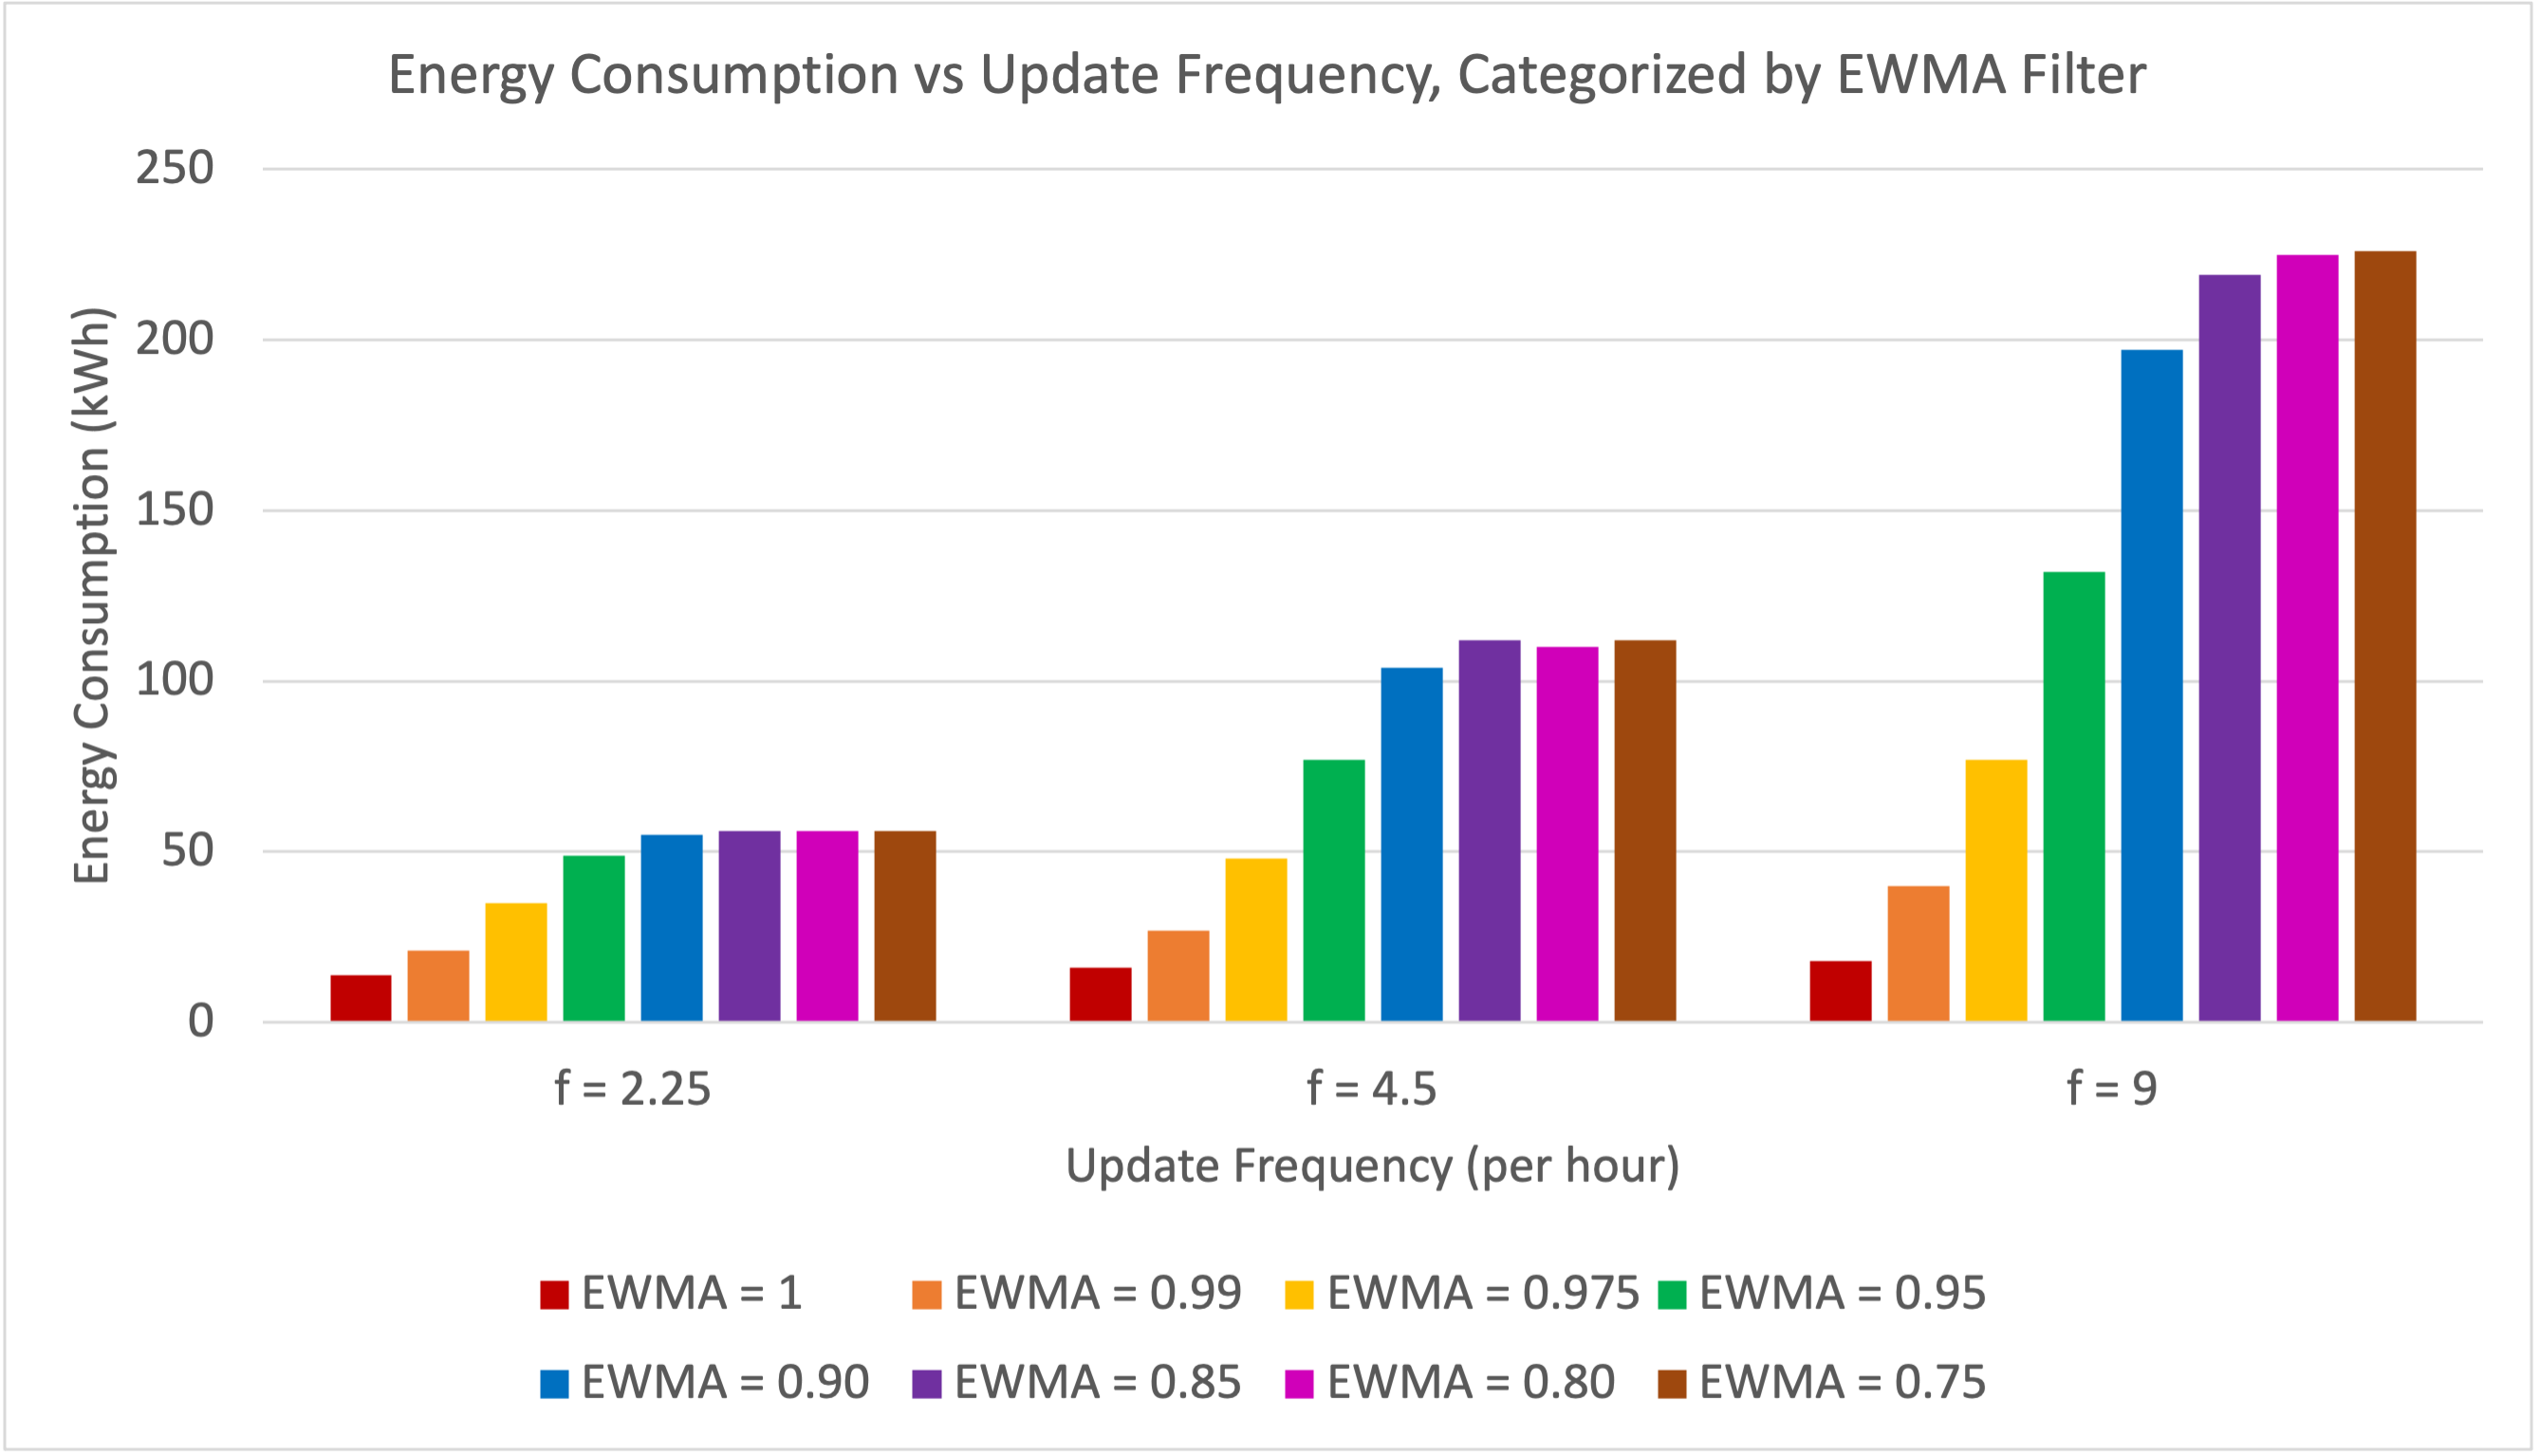
\includegraphics[scale=0.48]{barfreq.png}
    \caption{The energy consumption of the HVAC system versus the specified update frequency (per hour), color-categorized by the eight possible EWMA filters.}
\end{figure}
\begin{figure}[H]
    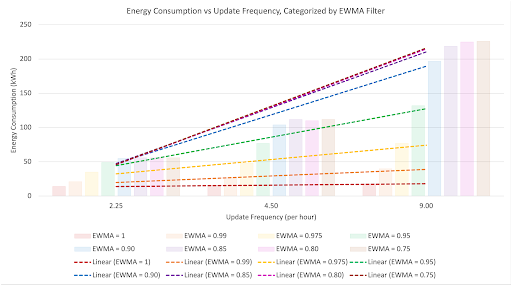
\includegraphics[scale=0.48]{linefreq.png}
    \caption{The trendlines of the energy versus update frequency graph, consisting of linear functions to represent the approximate trend of energy consumption with rising frequency, separated by EWMA filter.}
\end{figure}
These two figures can also lead to at least two conclusions:
\begin{enumerate}
\item For any specified EWMA filter, energy consumption increases as update frequency increases from 2.25 to 9 updates/hour. This energy increase somewhat resembles a linear function for our specifications, appearing to have a relatively consistent increase for each time we double the frequency. However, further studies with a wider range of frequencies (with each frequency being double the previous one, just how 4.5 is double of 2.25 and 9 is double of 4.5) would be necessary to be certain with this observation.
\item A lower EWMA filter leads to a greater dependence on frequency, meaning that the change in energy consumption is dependent on the combination of EWMA filter and update frequency. (This is very similar to the second conclusion of EWMA Impact.)
\end{enumerate}
\section{Conclusion}
\label{sec:Conclusion}

In conclusion to the simulation and the findings, we can conclude that by manipulating the EWMA filtering and the update frequency accordingly, i.e. increasing the EWMA filtering and decreasing the frequency, we can achieve significant energy and cost savings while also maintaining the average room temperature in the range of the setpoint temperatures, thus maintaining occupancy comfort. 

One of the downsides to this approach, however, is that the manipulation to these factors can account for longer response times, i.e. the time taken by the HVAC System to respond to setpoint changes accordingly. This is because if the controller activates the different heating/cooling chambers at a greater time interval, it would take longer in general for the HVAC system to quickly respond to a change in setpoints. 

Moreover, these findings give way to some future work, which we hope to research upon and implement. Firstly, we need to account for temperature setpoints being manipulated by the occupants on the thermostats. In other words, we need to factor in for changing setpoints throughout the day, and calculate an optimal response time.

The psychological aspects of the occupants who are in control of the thermostats also need to be accounted for, and we need to define "occupant comfort" in a more in-depth finer detail. Since the occupants are the main benefactors of the HVAC System in a typical commercial building, the psychological aspects of their comfort need to be taken into account.

We also plan to expand our current simulation to be able to account for more controller specifications outside of the Johnson Controls PRAC+ controllers. This would give us a wide range of dataset to analyze, as well as determine more alternative ways of energy and cost savings across a greater sample set of buildings.

\section{Acknowledgements}
We would like to thank the following people, who have aided us greatly in our research and our project development.
\begin{enumerate}
    \item Peter Volpe: Electrical Engineer, UMass CHP
    \item Fidele Mazimpaka: UMass Campus Energy Engineer
    \item Ted Mendoza: Capital Projects Manager, UMass Sustainability, and Carbon Zero
    \item UMass Central Heating Plant, and UMass Carbon Zero
    \item Professors Shira Epstein and Nick Tooker: iCons 3 Spring 2023 Instructors
    \item The iCons Program at the University of Massachusetts Amherst.
\end{enumerate}



\bibliographystyle{IEEEtran}
\bibliography{IEEEabrv,IEEEReferences}

\end{document}
